\documentclass{article}
\usepackage[hmargin=0.65in, vmargin=0.65in]{geometry}
\usepackage[utf8]{inputenc}
%% \usepackage{indentfirst}
\usepackage{listings}
\usepackage{xcolor}
\usepackage{hyperref}
\hypersetup{
    colorlinks=true,
    linkcolor=blue,
    filecolor=magenta,      
    urlcolor=cyan
    }
\usepackage{graphicx}
\graphicspath{ {./images/} }


\title{CS 470 Homework 1}
\author{Niki Vasan}
\date{February 2nd, 2023}

\begin{document}

\maketitle

\textbf{Collaboration Statement:} I did not collaborate with any peers on this assignment. However, I used online resources including sci-kit learn's documentation, stack overflow and stack exchange (particularly this \href{https://stackoverflow.com/questions/39421202/adding-a-grouped-by-zscore-column-to-a-pandas-dataframe}{post}), and a medium article on feature scaling techniques linked \href {https://towardsdatascience.com/data-normalization-with-pandas-and-scikit-learn-7c1cc6ed6475}{here}.

\section{Data Exploration and Pre-Processing}
\paragraph{\textbf{Task 1:}} The dataset has 29 columns. 
\begin{itemize}
    \item \textbf{Semester:} describes the semester the course was taken in. I would argue that semester is an ordinal variable. It is nominal, since its given form of SXX or FXX is not numeric, but it is a time-series ordered variable. F16 will always come before S17, which will always come before F17, etc. 
    \item \textbf{Student ID:} is the school-sponsored ID of the student. This is a nominal (categorical) variable, because even though the ID is composed of numbers, the values don't have any numeric relationship to one another, as they are usually randomly chosen
    \item \textbf{Name:} is a nominal variable representing the name of the student. 
    \item \textbf{Section:} is a nominal variable representing the section of the course the student is in. Again, although section is a number, there is no numeric relationships amongst the values. Furthermore, there is no ordering between the sections (i.e. Section 1 of CS170 is not better or worse than Section 2 of CS170). 
    \item \textbf{Homeworks 1-5:} represent the homework scores for each of the five homeworks, which are graded out of 40 points. Determining the type of attribute in this case can be a bit of a grey area depending on how grades are interpreted. If you interpret these grades with respect to their percentile equivalent, then they are ordinal attributes, since the difference between certain scores is not the same (i.e. a 90-80 measures a larger difference in ability compared to 20-10). If you interpret the scores as raw numbers, this is a numeric ratio-scaled variable because there is an inherent zero point. Because the scores are not explicitly written in percentiles or letter groups, I will assume the attribute is numeric ratio-scaled. 
    \item \textbf{Peer Evaluations:} are the total peer evaluation scores for each student, graded out of 150 points. This is a numeric ratio-scaled variable because it has real numbers as values and has an inherent 0 point.
    \item \textbf{Bonus:} accounts for bonuses students can receive for early submission and catching typos. Although each individual bonus has a discrete set of values (i.e. 2 for early submission, 1 for typos etc.), I am making the assumption each student can receive any number and any combination of these bonuses throughout the semester, making the attribute itself numeric. 
    \item \textbf{Quizzes 1-12:} describe the scores received on each of the 12 quizzes administered throughout the semester. The same analysis done on the "Homeworks" attribute applies here, meaning the attribute is a numeric ratio-scaled variable. 
    \item \textbf{Quiz Adjustments:} appear to represent adjustments to existing quizzes or makeup quizzes due to extenuating circumstances. This is a sparse numeric variable. 
    \item \textbf{Drop Lowest Quiz 1 and 2:} represent the scores of the lowest two quizzes for each student that are dropped from the total score. This is a numeric variable as it represents a quantity for subtraction.
    \item \textbf{Final Exam:} is the score students receive on their final exam for the class, which is out of 150 points. This attribute's values are integers. Again, similar to the Homework and Quiz attributes, this is a numeric ratio-scaled variable because there is an inherent zero. 
    \item \textbf{Total Score:} represents the total number of points each student has accumulated throughout the semester. This is a numeric ratio-scaled variable because it has an inherent zero point. 
    \item \textbf{Letter Grade:} is the letter grade corresponding to the Total Score attribute. This is an ordinal variable, as the values have a meaningful order (i.e. A+ $>$ A $>$ A- $>$ B+ etc.). 
\end{itemize}

\paragraph{\textbf{Task 2:}} 
\begin{itemize}
    \item \textbf{Homeworks 1-5:} These attributes have 18, 17, 26, 30 and 43 missing values per feature respectively. Dropping missing records will not be an option in this dataset as each student needs a final grade for the course UNLESS they drop the course entirely. To account for this, student IDs with missing values should be cross listed amongst the list of student IDs of those who dropped or withdrew from the course at any point during the semester. This applies for all attributes. These records should be automatically removed. Another interpretation is that students simply did not turn in the assignment. This interpretation also makes sense given that the number of missing values increases as the semester moves forward, aligning with student burnout and course withdrawal. Under this assumption, all missing values should be imputed with zeros, as the assignment was not turned in. However, this may not be a foolproof solution, as it is unclear whether QTest or Canvas would automatically score missing assignments as a zero. There appear to be a few rows where one or more of the Homework scores are 0, which could mean the student either had a submission that yielded 0 points or did not submit anything at all. If it is indeed true that a 0 represents an unsubmitted assignment, then another possible cause of the missing values is due to error (perhaps QTest or Canvas went down). In these specific instances, it is likely best to manually fill in the correct score if the student has proof or a record of the score they received, or give them full points, although this might be a tedious process. 
    \item \textbf{Peer Evaluations:} This attribute has 40 missing values. All students who dropped the course should be removed. Again, it is unclear whether the grading system used would automatically impute missing assignments as 0. Given that there are no true 0 values in this feature, it is likely that these missing values represent students who did not submit any peer evaluations or an error on the part of the grading system. In this case of incomplete assignments, all values should be imputed with a 0. In the case of machine error, there are a few solutions. One could be simply imputing the median peer evaluation score. This is a simple, time-efficient solution but may unfairly penalize high performing students who would have otherwise gotten a score above the 50th percentile. A more accurate way to impute this value is to train a regression model using the other assignments as predictors, so that each student will get a score in alignment with other students who have had similar performance on other assignments. However, this is more computationally expensive and required more time and effort.
    \item \textbf{Bonus:} The Bonus feature is sparsely populated since the bonus is an optional assignment. Missing values likely mean students who didn't submit a homework assignment early or catch a typo. This means that all missing values should simply be imputed with a 0, as not completing a bonus should not positively or negatively affect the final score. 
    \item \textbf{Quizzes 1-12:} The quizzes should be handled similarly to the Homeworks. There appears to be a distinction in the data between 0s and missing values. This might mean that a 0 represents a submitted, completely incorrect assignment, or it could mean an unsubmitted assignment and the other missing values are due to machine error. Without more context on the grading system used, it is difficult to determine the source of error. If all missing values are unsubmitted assignments, they should all be imputed with a 0. If they are due to machine error, all students who have a record of their score after submission should have their scores manually inputted. Everyone else could either have the median inputted or a regression model could be trained to predict their scores with the other assignments as the predictors. The pros and cons of this were discussed above.
    \item \textbf{Quiz Adjustment:} Given the sparsity of this feature, it seems reasonable to assume that adjustments only apply to a small number of students and that the students who do not require an adjustment do not incur a penalty. For this reason, it is likely the most efficient to impute all missing values with 0s.
    \item \textbf{Drop Lowest Quiz 1 and 2:} These attributes do not have any missing values.
    \item \textbf{Final Exam:} There are 41 missing values in this attribute. When filtering for these records, it is clear that many of these records represent students who dropped the course, as many of the previous assignments leading up to the final are also missing. As mentioned before these records should be dropped. There also are no records with the value 0 for this attribute, which means these missing values are likely due to an unsubmitted final and can be imputed with a zero. Any special cases of machine error should be handled with manual imputation although tedious, as mentioned before. 
    \item \textbf{Total Score and Letter Grade:} These attributes have no missing values.
\end{itemize}

\paragraph{\textbf{Task 3:}} 
\indent The attributes \textit{Semester} and \textit{Section} are not encoded very well. \textit{Semester} is represented by F or S concatenated with the year (16,17,18). Because it begins with a letter, when you use python's native sorting functions, all the Fall semesters will alphabetically come before the Spring semesters, which is not in chronological order. \textit{Section} needs to be re-encoded as well because it is inconsistent. Semester F16 does not have a Section 5, while Semesters F17 and F18 do not have a Section 0. The Spring sections only have 6 sections compared to nine in the fall, but S17 goes from 0-5 while S18 goes from 1-6. This makes it difficult to make time series comparisons across the data. 

Given that there are only 5 semesters in this dataset, one way of re-encoding \textit{Semester} is to simply number the semesters from 1 to 5 in the correct chronological order, making sure to clearly document the mapping (e.g. F16 = 1, S17 = 2, etc.). This would ensure that the data will always be sorted chronologically, which will facilitate time series analyses. \textit{Section}'s numbering simply needs to be standardized. The Fall Semesters should be from 1-9 consecutively and the Spring semesters should be from 1-6.

Below is the code used to recode the \textit{Semester} attribute using the \textit{pandas} package in Python. 

    \begin{lstlisting}[language=Python]
    import pandas as pd
    
    data['Semester'] = data['Semester'].str.replace('F16', '1')
    data['Semester'] = data['Semester'].str.replace('S17', '2')
    data['Semester'] = data['Semester'].str.replace('F17', '3')
    data['Semester'] = data['Semester'].str.replace('S18', '4')
    data['Semester'] = data['Semester'].str.replace('F18', '5')
    
    data.sort_values(by=['Semester'], inplace=True)
    data['Semester'] = data['Semester'].astype("int")
    \end{lstlisting}

Here is the code used to recode the \textit{Section} attribute.
    \begin{lstlisting}[language=Python]
    # Re-encode Section 1 (F16)
    import pandas as pd
    
    mapping1 = {0:0.5, 1:1.5, 2:2.5, 3:3.5, 4:4.5, 6:6.5, 7:7.5, 8:8.5, 9:9.5}
    data[data['Semester'] == 1] = 
    data[data['Semester'] == 1].assign(Section = 
        data[data['Semester'] == 1].Section.map(mapping1))
    mapping2 = {0.5:1, 1.5:2, 2.5:3, 3.5:4, 4.5:5, 6.5:6, 7.5:7, 8.5:8, 9.5:9}
    data[data['Semester'] == 1] = 
    data[data['Semester'] == 1].assign(Section = 
        data[data['Semester'] == 1].Section.map(mapping2))
    print(data[data['Semester'] == 1]['Section'].unique(),
        len(data[data['Semester'] == 1]['Section']))
    
    # Re-encode Section 2 (S17)
    import pandas as pd
    
    data.loc[data['Semester']== 2,'Section'] = data['Section'] + 1
    data[data['Semester'] == 2]['Section'].unique()
    \end{lstlisting}


\paragraph{\textbf{Task 4:}} 
There are 20 attributes in the data that represent a score, including: Homeworks 1-5, Peer Evaluations, Quiz 1-12, Final Exam and Total Score. The Bonus and Quiz Adjustment columns are sparse, so I will not be scaling them.
\begin{enumerate}
    \item \textbf{Min-Max Normalization:} The first task asks us to rescale the attributes on the interval between 0 and 100. There are two approaches to this. One option is to use the maximum score found in the data with a standard min-max normalization. Another option is to rescale the entire attribute to where the min is 0 and the max is 100. I think it is important to scale all attributes on the same range ([0,100] because differing scales can impact the fitting of models that are sensitive to feature scaling. To accomplish this in Python, I used the Min-Max Scaler class available in sci-kit learn. 
    \begin{lstlisting}[language=Python]
    from sklearn.preprocessing import MinMaxScaler
    
    df = data.iloc[:,[4,5,6,7,8,9,11,12,13,14,15,16, 17,18,19,20,21,22,26,27]]
    scaler = MinMaxScaler([0,100])
    data_norm = pd.DataFrame(scaler.fit_transform(df), columns=df.columns)
    col_names = [col + ' MM' for col in data_norm.columns]
    data_norm.columns = col_names
    data_copy = pd.concat([data, data_norm], axis=1)
    data_copy.head()
    \end{lstlisting}
    \item \textbf{Z-Score Method:} The second task requires using the z-score normalization, which transforms the data into a distribution where the mean is 0 and the standard deviation is 1 
    ($z = x - \mu / \sigma$). To accomplish this, I used the Standard Scaler class available in sci-kit learn, which may differ slightly from a manual implementation because it uses the population standard deviation (N) instead of the sample standard deviation (N-1).
    \begin{lstlisting}[language=Python]
    from sklearn.preprocessing import StandardScaler
    
    df = data.iloc[:,[4,5,6,7,8,9,11,12,13,14,15,16, 17,18,19,20,21,22,26,27]]
    scaler = StandardScaler()
    data_norm = pd.DataFrame(scaler.fit_transform(df), columns=df.columns)
    col_names = [col + ' ZS' for col in data_norm.columns]
    data_norm.columns = col_names
    data_copy2 = pd.concat([data_copy, data_norm], axis=1)
    data_copy2.head()
    \end{lstlisting}
    \item \textbf{Z-Score Method (By Semester):} The third task is the same as above, but instead we will be using the mean and standard deviation of students in the same semester. I used a manual implementation of z-score normalization here using pandas, ensuring to keep the standard deviation as the population standard deviation used in the sklearn implementations above.
    \begin{lstlisting}[language=Python]
    import pandas as pd
    
    df2 = data.iloc[:,[0,4,5,6,7,8,9,11,12,13,14,15,16,17,18,19,20,21,22,26,27]]
    z_score = lambda x: (x - x.mean()) / x.std(ddof=0)
    for col in df2.columns[1:]: 
        new_col = col + ' ZSG'
        df2.insert(len(df2.loc[0]), new_col, df2.groupby(['Semester'])[col].
        transform(z_score))
    df2 = df2.filter(regex=('ZSG$'))
    df2.columns
    data_copy3 = pd.concat([data_copy2, df2], axis=1)
    data_copy3.head()
    \end{lstlisting}
    \item \textbf{Discussion:} These techniques have advantages and disadvantages that may make them best suited for different contexts. The min-max normalization is helpful because it means all the assignments are scored at the same scale, which facilitates pairwise comparisons and is a necessary prerequisite for models that are sensitive to feature scale. However, it is very sensitive to outliers, which are plenty in this dataset. This means if this technique were to be used, it would probably be a good idea to remove any outliers first. The Z-Score standardization is useful because it accounts for both the mean and variability in the data. It allows for direct comparison of variables with different scales and means, which is especially helpful in the case of this dataset where the Final Exam is out of 150 points, for example, but the Homeworks are only out of 40. However, it does assume a normally distributed curve, which is not always a given. You also lose the interpretability of the raw attribute values. Because of this, the z-score transformation might be helpful when training a model, for example, but maybe not for descriptive cuts of the data or creating visualizations. The grouped z-score might be helpful if doing a time-series analysis where the data will be compared by semesters, as it ensures the scores are generated only from the pool of students in a given semester. This would ensure the distribution is robust against any irregularities such as the pandemic or teaching issues that could have occurred in a specific semester. 
    
\end{enumerate}
 
\paragraph{\textbf{Task 5:}} I calculated the 5-number summary, mean and standard deviation for the 20 variables I mentioned in Task 4 as well as for their scaled counterparts. In this document, I will only include the summary table for the raw (unscaled) attributes, but the code to produce all the statistics for every score attribute is below. 
    \begin{lstlisting}[language=Python]
    import pandas as pd 
    
    d3 = data_copy3
    cols = pd.Series(d3.columns)
    cols = cols.loc[cols.str.startswith(('Homework', 'Quiz', 'Peer', 'Final Exam', 
    'Total Score'),na=False)]
    cols = cols.drop(23) # remove Quiz Adjustment
    d3 = d3[cols]
    # summary table for all 80 attributes
    summary = round(d3.describe().loc[['min', '25%', '50%', '75%', 'max', 'mean', 'std']],2) 
    # summary for original (unscaled) features
    summary.iloc[:,:20] 
     \end{lstlisting}

    \includegraphics[scale=0.6]{summary1.png}
    
    \includegraphics[scale=0.6]{summary2.png}

\paragraph{\textbf{Task 6:}} Below are the charts generated from the data. First, here are three boxplots representing the distribution of the first, third and fifth homeworks. We can see that Homework 3 has the largest variance and most significant outliers, likely representing students who have dropped the course or may be struggling over time. Homework 2 has the smallest interquartile range, thus indicating students performed relatively better on this assignment. However, the medians for the three assignments are still all relatively similar. We can also see the outliers all abnormally low, which makes sense because there aren't extremely significant (+10 points for example) bonuses available to make these homework grades abnormally high.


\includegraphics[scale=0.6]{boxplots.png}

Below are histograms demonstrating the distribution of letter grades for the final exam for the first three semesters. The first graph measures the percent of total students who fall into each letter chart, and the second chart measures the raw count. From the second chart, we can see on average that the fall semesters have higher enrollment than the spring semesters, which makes sense given that this is a prerequisite course for all CS courses. From the first chart, we can see that Spring 2017 has the percentage of As out of all the semesters, which may be due to sheer chance or increased variability in scores due to lower total enrollment. One interesting observation is that the distributions of Spring 2018 and Fall 2018 are almost identical and have higher scores on average. This could be due to consistent teaching/grading or strong batches of students. 

\hspace*{-1.5cm}  
    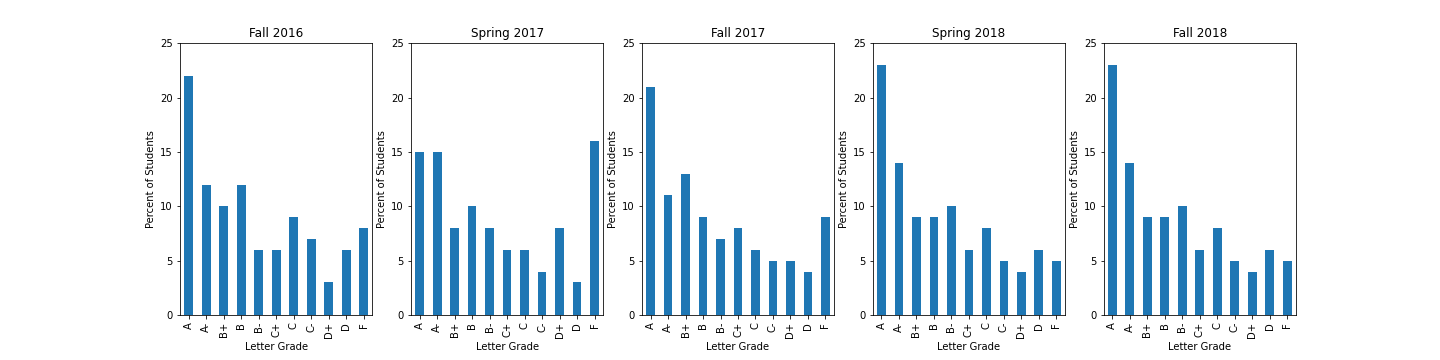
\includegraphics[scale=0.4]{histograms-percent.png}

\hspace*{-1.5cm}  
    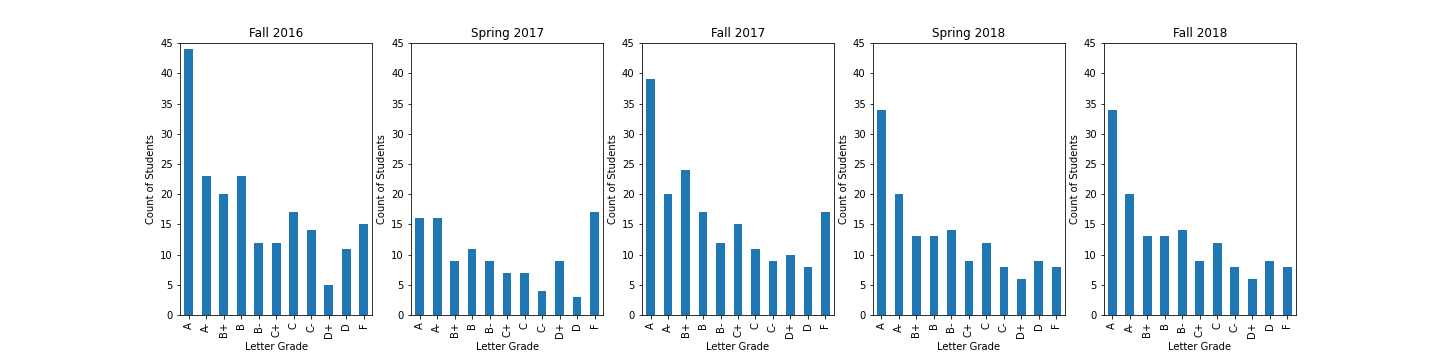
\includegraphics[scale=0.4]{histograms.png}


Lastly, below are three scatterplots that aim to observe  what assignments are most correlated with the students' total score for the course: Average Quiz Score (derived from the quiz attributes), Average Homework Score (derived from the homework attributes) and Final Exam Score. The plots are also stratified by the season the course takes place in (Fall or Spring). Out of three variables, the average quiz score appears to be most linearly correlated with total score, but all three assignments are generally positively correlated with the overall score for the class. There does not appear to any significant difference in the season the course was taken in. 

\hspace*{-2.6cm}  
    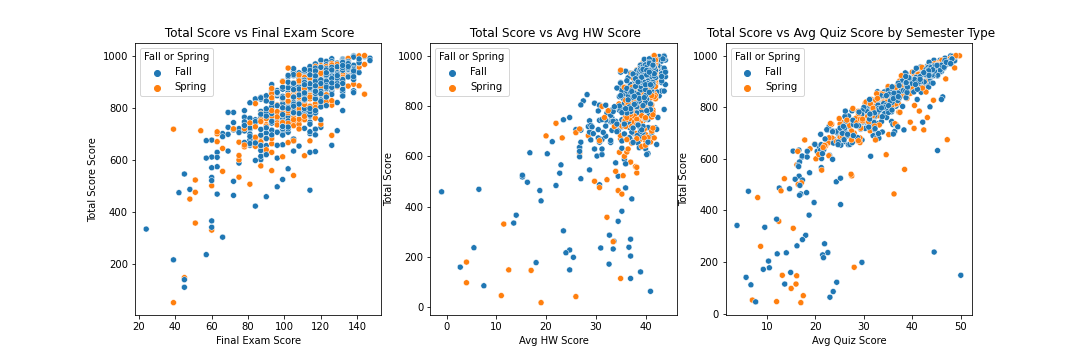
\includegraphics[scale=0.6]{scatterplots-updated.png}

\paragraph{\textbf{Task 7:}} The only tool I used for this project was Python (pandas, numpy, sklearn, seaborn, matplotlib). I used a jupyter notebook to clean, format, export and visualize the data. However, when re-encoding the Sections in Part 3, I found it helpful to make some of the changes in Excel first just so I could visualize the logic, and then I was able to write a code to automate the process in Python. Excel was more intuitive to use, particularly when trying to account for a missing number in the Section labeling, but it is tedious to use for larger datasets. When doing feature scaling, I originally manually wrote code to do the normalization, but later realized it was much more efficient to use sklearn built-in Min-Max and Standard Scaler classes. However, although using libraries saves  time, it is difficult to customize, so for 3 in Task 4 that asked for normalizing based on Semester, I ended up writing my own code. 

\end{document}
